\section{Clustering en el espacio eucl\'ideo}

En la secci\'on anterior presentamos algunos de los inconvenientes te\'oricos 
del m\'etodo propuesto por Moreno-Dominguez. A continuaci\'on mostramos como 
solucionar todos ellos haciendo uso de la tranformaci\'on \textit{logit}. \\

\subsection{Transformaci\'on Logit}
\label{sec:logit}

Sea $P_M$ el espacio de una distribuci\'on discreta para $M$ etiquetas: 

$$P_M = \left\{  p | p = (p_1,\dots p_n) \in (0,1)^M , \sum{p_i} = 1 \right\}$$

La funci\'on \textit{logit}:$P_M \rightarrow R^{M-1}$ define una transformaci\'on
entre el espacio $P_M$ y el espacio eucl\'ideo $R^{M-1}$. Dados los vectores $Q \in P^M$ y
$S \in R^{M-1}$:

$$S_i = logit(Q_i) = log\left(\frac{Q_i}{Q_M}\right)$$

Para el caso de $M=2$ permite transformar la distribuci\'on Bernoulli
discreta al espacio eucl\'idio. Podemos ver en la ecuaci\'on \ref{eq:logit} su
expresi\'on anal\'itica y en la Figura \ref{fig:dominio} representaci\'on 
gr\'afica.

\begin{figure}[h!]

\begin{minipage}[b]{0.45\textwidth}

    \begin{equation}
    \vspace{2.85cm}
        \label{eq:logit}
    logit(p) = log\left(\frac{p}{1-p}\right)
    \end{equation}
\end{minipage} ~
\hfill
\begin{minipage}[b]{0.45\textwidth}
    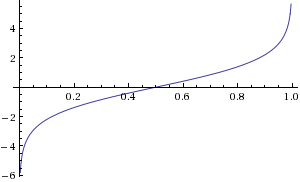
\includegraphics[width=\textwidth]{img/logit.png}
    \caption{Representaci\'on gr\'afica de la funci\'on logit}
    \label{fig:dominio}
\end{minipage} ~

\end{figure}  

Trabajar en el espacio eucl\'ideo nos asegura que la suma y la multiplicaci\'on
por escalares est\'an contenidos en el mismo espacio. Pohl et al. \cite{Pohl2007} 
utilizan esta propiedad para realizar operaciones lineales sobre mapas
probabil\'isticos. A su vez, demuestran que la suma y multiplicaci\'on
por escalares en el espacio eucl\'ideo poseen un significado en el espacio de la
distribuci\'on. \\

\subsection{Modificando el algoritmo de clustering}
\label{sec:modificandoClustering}

Asumiendo que cada voxel $v$ de un tractograma proviene de la variable 
aleatoria binaria:

 $$X_v= \textrm{``La semilla est\'a conectada con el voxel v''}$$
 
Es posible transformar el tractograma aplicando la funci\'on \textit{logit} en
cada uno de sus voxels. El resultado es un vector donde cada coordenada se 
encuentra en el espacio eucl\'ideo. M\'as a\'un, las operaciones lineales entre
los mismos voxels en distintos tractogramas est\'an definidas. Esto nos permite
usar la m\'etrica eucl\'ideana como funci\'on de similitud en \textit{Agglomerative
Hierarchical Clustering}. \\

Transformar de espacio los tractogramas y cambiar la funci\'on de similitud 
posee varias ventajas. Para empezar permite agrupar correctamente vectores
colineales. La Figura \ref{fig:3logit} muestra el resultado de aplicar este
m\'etodo a los vectores de la Figura \ref{fig:3clusters}. Podemos apreciar 
que las tres poblaciones se encuentran correctamente separadas y bien definidas.\\

\begin{figure}[h!]

\centering
\begin{minipage}[b]{0.85\textwidth}
    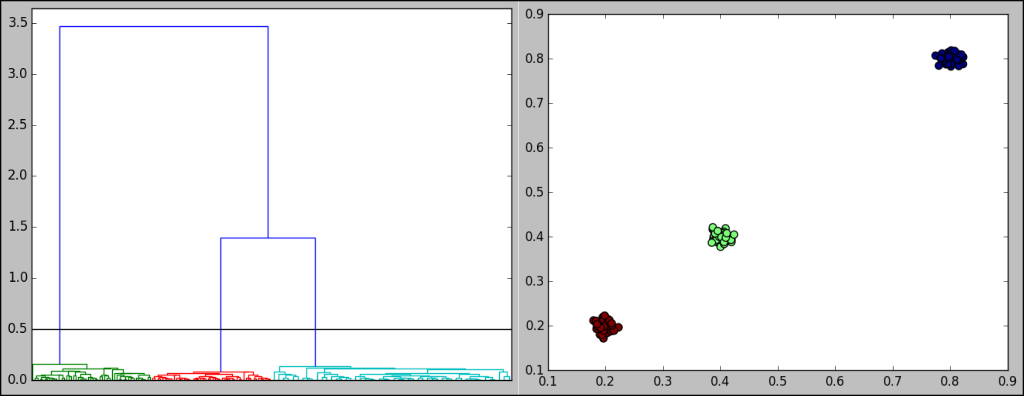
\includegraphics[width=\textwidth]{img/3pop_logit.png}
    \caption{Clustering resultado de utilizar el m\'etodo logit}
    \label{fig:3logit}
\end{minipage} ~

\end{figure}  

Otra ventaja es la buena relaci\'on m\'etrica-\textit{linkage}. Por definici\'on
el centroide es el centro de masa de los clusters. Esto quiere decir que es el 
punto que minimiza la distancia euclidiana entre los clusters que lo componen. 
Por ende, el centroide caracteriza bien el punto medio de los vectores en el
espacio eucl\'ideo. \\

Finalmente, nuestro m\'etodo tambi\'en permite mejorar la complejidad algor\'itmica.
Como ya explicamos, por cada iteraci\'on del algoritmo 
\textit{Agglomerative Herarchical Clustering} es necesario calcular un representante
de la uni\'on y luego computar su distancia al resto. Sin embargo, al usar la
m\'etrica euclideana junto con el \textit{linkage} centroide es posible simplificar
este paso. \\

\begin{equation}
\label{eq:lyw}
d(i \cup j,k) = \alpha_i d(i,k) + \alpha_j d(i,k) + \beta d(i,j) + \gamma | d(i,k) - d(j,k) |
\end{equation}

\begin{equation}
\label{eq:lyw2}
\alpha_i = \frac{|i|}{|i|+|j|} \hspace{0.5cm}
\alpha_j = \frac{|j|}{|i|+|j|} \hspace{0.5cm}
\beta = -\frac{|k|}{|i|+|j|+|k|} \hspace{0.5cm}
\gamma = 0
\end{equation}

\hspace{0.5cm}

La formula de Lance y Williams (ecuaci\'on \ref{eq:lyw}) permite computar
las nuevas distancias sin comparar expl\'icitamente los clusters. Para el m\'etodo
centroide los parametros son las relaciones de la ecuaci\'on \ref{eq:lyw2}. Usar esta formula reduce
significativamente la complejidad. Cada iteraci\'on pasa a costar $O(c^2)$ en 
vez de $O(c^2 m)$, siendo $c$ la cantidad de clusters y $m$ la longitud de los
mismos. Dadas $n$ semillas iniciales, la complejidad temporal total del
\textit{clustering} es $O(n^3)$.  Con la distancia coseno era $O(n^3 m)$, siendo
$m$ la longitud de los tractogramas. Recordemos que en el contexto en que estamos
 utilizando este algoritmo $m>>n$. Por
lo tanto, este resultado implica una gran mejora en la eficiencia del algoritmo.  
